\documentclass{article}

% set font encoding for PDFLaTeX or XeLaTeX
\usepackage{ifxetex}
\ifxetex
  \usepackage{fontspec}
\else
  \usepackage[T1]{fontenc}
  \usepackage[utf8]{inputenc}
  \usepackage{lmodern}
\fi
\usepackage{graphicx}
% used in maketitle
\title{Reporte de Actividad 2}
\author{Rolando A. Fimbres G.}
\date{8 de Febrero, 2018}

% Enable SageTeX to run SageMath code right inside this LaTeX file.
% documentation: http://mirrors.ctan.org/macros/latex/contrib/sagetex/sagetexpackage.pdf
% \usepackage{sagetex}

\begin{document}
\maketitle

\section{Introducción}
La actividad realizada trato acerca de cómo analizar una base de datos desde el entorno \textit{Jupyter Notebook} utilizando el lenguaje python. Para poder desarrollar la actividad recurrimos a extraer una base de datos de una estación del servicio meteorológico nacional. En mi caso el lugar escogido fue el de los Lagos de Montebello en el estado de Chiapas.\\
Después de descargar los datos, se nos pidió replicar los códigos de un ejemplo proporcionado. Éstos códigos se encargaron de analizar los datos de distintas maneras tales como gráficas relacionando sus características. 

\begin{figure}[h!]
    \centering
    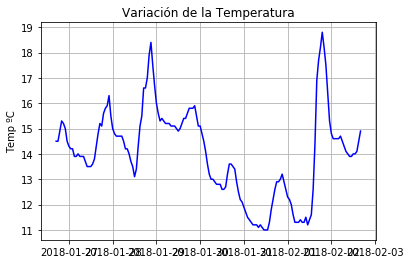
\includegraphics[width=\linewidth]{vt_vs_t.png}
\end{figure}

\begin{figure}[h!]
    \centering
    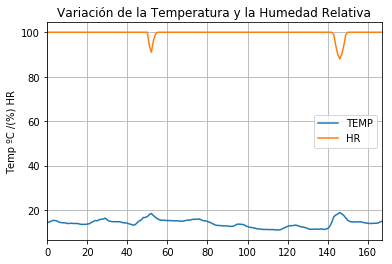
\includegraphics[width=\linewidth]{vthr.png}
\end{figure}

\begin{figure}[h!]
    \centering
    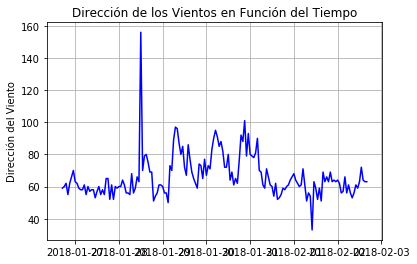
\includegraphics[width=\linewidth]{dv_vs_t.png}
\end{figure}

\begin{figure}[h!]
    \centering
    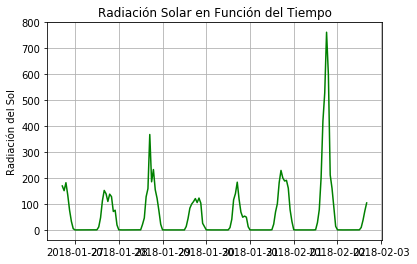
\includegraphics[width=\linewidth]{rs_vs_t.png}
\end{figure}

\begin{figure}[h!]
    \centering
    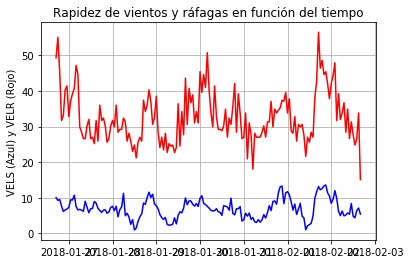
\includegraphics[width=\linewidth]{rvrr_vs_t.png}
\end{figure}

\begin{figure}[h!]
    \centering
    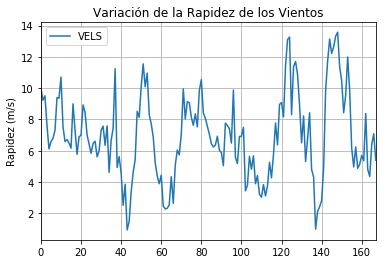
\includegraphics[width=\linewidth]{vrv_vs_t.png}
\end{figure}

\section{Apéndice.}
1.-¿Cuál es tu primera impresión de Jupyter Notebook?\\
Me gustó el diseño, así era como me imaginaba una especie de editor en linea.\\
2.-¿Se te dificultó leer código en Python?\\
La verdad es que no, yo esperaba que resultara difícil para mi, pero una vez que prestas atención y lo relacionas con lo que conoces es fácil.\\
3.-¿En base a tu experiencia de programación en Fortran, que te parece el entorno de trabajar en Python?\\
Me parece más cómodo pues verificar si el código funciona es más rápido.\\
4.-A diferencia de Fortran, ahora se producen las gráficas utilizando la biblioteca de Matplotlib. ¿Cómo fue tu experiencia?\\
Me gustó pues me parece más sencilla la forma de obtener gráficos.\\
5.-En general, ¿qué te pareció el entorno de trabajo en Python?\\
Me pareció agradable, más sencillo y fácil de corregir y editar.\\
6.-¿Qué opinas de la actividad? ¿Estuvo compleja? ¿Mucho material nuevo? ¿Qué le faltó o que le sobró? ¿Qué modificarías pára mejorar?\\
Me gustó. Aunque no conocía muchas cosas fue fácil adaptarse. Me parece que tuvo lo adecuado.\\
7.-¿Comentarios adicionales que desees compartir?\\
Aunque me pareció fácil, tomé algo de tiempo para llegar a terminarlo por completo.\\

\end{document}
